\chapter{Estrutura}

\section{Requisitos}

Os requisitos de para a estrutura são:


\begin{itemize}
\item A estrutura deve suportar o peso de todos os componentes com margem de segurança para eventuais cargas não estimadas;
\item Deve possuir resistência a ação climática, especificamente a radiação solar, temperatura elevada e corrosão devido a exposição a chuva;
\item A placa solar que fornece a energia do sistema deve ficar oposta a caixa de painel de controle superior;
\item Os sistemas de antena e câmera devem estar em montantes articulados a 3 metros de altura para que a incidência possa ser ajustada e mais eficiente;
\item A estrutura deve conter suporte para manutenção facilitada, permitindo o acesso aos componentes de maneira facilitada;
\item O vento incidente devido a região de instalação deve também ser suportado pela estrutura;
\end{itemize}

\section{Restrições}

As restrições de para a estrutura são:

\begin{itemize}
\item Os materiais não podem ser suscetíveis a corrosão, a ruptura por radiação e temperatura solar para não comprometer o funcionamento dos sistemas eletrônicos;
\item A estrutura não pode ter área de contato com o vento muito elevado;
\item Os compartimentos de instalação dos eletrônicos não pode possuir entrada para água ou detritos externos;
\item Os compartimentos não podem estar totalmente isolados, permitindo acesso para reparos e manutenção;
\item Os materiais selecionados não podem impedir o funcionamento de qualquer um dos componentes eletrônicos, a exemplo de impedir a emissão ou recepção do radar.
\end{itemize}

\section{Riscos}

Os riscos encontrados para o projeto de estrutura são:

\begin{itemize}
\item RSN 1 - Atrasos por fornecimento de materiais;
\item RSN 2 - Montagem mal feita;
\item RSN 3 - Interferência da estrutura com os equipamentos de radiofrequência;
\item RSN 4 - Atrasos causados por problemas de simulações e modelagem;
\item RSN 5 - Curto circuito de componentes eletrônicos causados pela estrutura;
\item RSN 6 - Dimensionamento errado;
\item RSN 7 - Fatores climáticos extremos.
\end{itemize}

%\section{Custos}

%Um levantamento orçamentário foi feito para a compra do material de construção do RaDop. Os custos aqui apresentados foram feitos através de contato com os fornecedores. 

%\begin{table}[H]
%\centering
%\resizebox{\textwidth}{!}{%
%\begin{tabular}{|c|c|c|c|c|}
%\hline
%\multicolumn{5}{|c|}{Estrutura}                                                                                     \\ \hline
%Quantidade & Material                                             & Valor Unitário & Total        & Fornecedor      \\ \hline
%2          & Caixa Para Painel Elétrico de Aço – 500x500x250m$^3$ & R\$ 240,00     & R\$ 480,00   & Soma            \\ \hline
%2          & Tubo Aço Carbono \#13 6m 2" 2,25mm                   & R\$ 105,24     & R\$ 210,48   & Perfibraz       \\ \hline
%4          & Barra Chata \#13 450x60mm$^2$                        & R\$ 12,00      & R\$ 48,00    & Perfibraz       \\ \hline
%4          & Barra Chata \#13 486x40mm$^2$                        & R\$ 12,00      & R\$ 48,00    & Perfibraz       \\ \hline
%2          & Barra Chata \#13 450x120mm$^2$                       & R\$ 22,00      & R\$ 44,00    & Perfibraz       \\ \hline
%1          & Barra Chata \#13 500,8x50,8mm$^2$                    & R\$ 13,30      & R\$ 13,30    & Perfibraz       \\ \hline
%1          & Tubo Quadrado 200x200mm$^2$ \#18 6m                  & R\$ 27,00      & R\$ 27,00    & Perfibraz       \\ \hline
%2          & Mão de Obra - Soldador                               & R\$ 50,00      & R\$ 100,00   & UnB             \\ \hline
%8          & Parafuso M5 Francês                                  & R\$ 0,25       & R\$ 2,00     & Líder           \\ \hline
%8          & Rosca M5                                             & R\$ 0,13       & R\$ 1,00     & Líder           \\ \hline
%16         & Parafuso M5 Sextavado                                & R\$ 0,15       & R\$ 2,40     & Líder           \\ \hline
%20         & Rosca M6                                             & R\$ 0,28       & R\$ 5,56     & Ferragens Lobão \\ \hline
%20         & Parafuso M6 Sextavado                                & R\$ 0,28       & R\$ 5,56     & Ferragens Lobão \\ \hline
%8          & Abraçadeira Tipo Copo Horizontal 1,5"                & R\$ 2,60       & R\$ 20,80    & Líder           \\ \hline
%1          & Cooler 120mm Led Ring Pc Gamer Fan                   & R\$ 58,80      & R\$ 58,80    & Mercado Livre   \\ \hline
%1          & Cimento Tocantins 50 Kg                              & R\$ 21,90      & R\$ 21,90    & Guarani         \\ \hline
%2          & Saco de Areia Média Lavada 30 Kg                     & R\$ 3,60       & R\$ 7,20     & Guarani         \\ \hline
%1          & Saco de Brita 30 Kg                                  & R\$ 3,60       & R\$ 3,60     & Guarani         \\ \hline
%2          & Cano PVC Metro 3" Branco                             & R\$ 9,00       & R\$ 18,00    & Guarani         \\ \hline
%1          & Mão de Obra - Pedreiro                               & R\$ 150,00     & R\$ 150,00   & UnB             \\ \hline
%2          & Suporte Articulado                                   & R\$ 45,35      & R\$ 90,70    & Mercado Livre   \\ \hline
%5          & Eletroduto Kanaflex Corrugado 1"                     & R\$ 2,90       & R\$ 14,50    & Japão Ferragens \\ \hline
%1          & Silicone Acético Incolor 280g                        & R\$ 14,90      & R\$ 14,90    & Japão Ferragens \\ \hline
%Descontos  & - -                                                  & - -            & R\$ 44,48    & - -             \\ \hline
%TOTAL      & - -                                                  & - -            & R\$ 1.328,32 & - -             \\ \hline
%\end{tabular}%
%}
%\caption{Custos dos materiais para a estrutura.}
%\label{custosestruturas}
%\end{table}

\section{Solução}

Utilizou-se o software CATIA V5 para a criação do CAD (\textit{computer aided design}) da estrutura. A estrutura completa e seus módulos separados foram construídos com base nas medidas das caixas comerciais e hastes selecionadas. Além disso, as medidas também foram baseadas para seguir uma proporção com os painéis solares. 

Temos o suporte principal para acoplar dos demais módulos da estrutura que foi chamada de hastes. Elas consistem em dois tubos de aço carbono afastados entre si a uma distância de 450 mm. Seu desenvolvimento foi pensado de forma a garantir a estabilidade da estrutura, por isso é possível ver a utilização de barras chatas de aço soldadas nas hastes para que a rigidez do sistema aumente.

A caixa superior é o local onde os componentes eletrônicos ficaram. Toda a transferência de dados acontece a partir dela. Os componentes vão possuir um espaço de 450x450mm em uma placa de montagem para seus devidos acoplamentos. Um \textit{cooler} foi instalado na lateral interna da caixa superior para ajudar na dissipação do calor. Em sua porta está fixado um holofote que serve de sinal luminoso para o motorista. Ambas as caixas possuem trancas para evitar a abertura de forma a expor os componentes a possíveis danos. 

A caixa inferior foi apoiada no chão pois a mesma carrega as baterias que alimentam energeticamente o sistema. Por questões técnicas, pois poderiam gerar um momento maior na base da estrutura devido ao braço de alavanca entre a caixa superior e o chão. A caixa inferior está ligada através de 4 abraçadeiras do tipo copo às hastes de suporte principal.

O suporte para o acoplamento dos painéis solares se encontra atrás da caixa superior. Este suporte foi soldado nas hastes em 4 pontos com uma angulação de 15 graus como solicitado pelo subsistema de energia para melhor captação de luz solar. 

No ponto mais alto da estrutura, a 3 metros do chão, temos dois componentes de suma importância para o funcionamento do RaDop. As antenas do radar Doppler e a câmera. A câmera possui três um grau de liberdade, o que permite a capturar com eficiência as imagens dos carros. Oposta à câmera e acima da caixa superior teremos duas antenas do radar Doppler. Elas possuem um suporte articulado que permite à elas três graus de liberdade, visando melhorar o apontamento das antenas para que a emissão e recepção do sinal sejam feitas da melhor maneira possível.

As plantas geradas a partir do \textit{software} CATIA V5, com detalhes em padrão internacional que foram utilizadas para a construção de todas as peças da parte estrutural, se encontram no Apêndice \ref{plantas_construcao} desse relatório, assim como as demais peças que não são do subsistema estrutural mas foram necessárias para dimensionar os módulos estruturais.

\subsection{Análise estática estrutural}

A força dinâmica causada pela força do vento foi calculada segundo a norma NBR 6123 (jun/88) \cite{ventos} e foram aplicadas à estrutura como cargas pontuais e constantes. O valor do vento para o projeto, também retirado da norma, é de 6 m/s.

Para a modelagem do problema foi considerado uma estrutura simétrica, e a tensão admissível pelos componentes estruturais é a tensão de escoamento do aço levando em consideração um fator de segurança. O material usado para o cálculo foi o aço carbono
com a tensão de escoamento no valor de 200 MPa \cite{callister}. Estimando o peso de cada componente em Catia e utilizando a metodologia para os cálculos de tensão principais \cite{beer}, foi possível determinar os esforços na estrutura.

A Figura \ref{fig:matlab} mostra o diâmetro mínimo que a estrutura deve ter para suportar os esforços estruturas.

        \begin{figure}[H]
	        \centering
            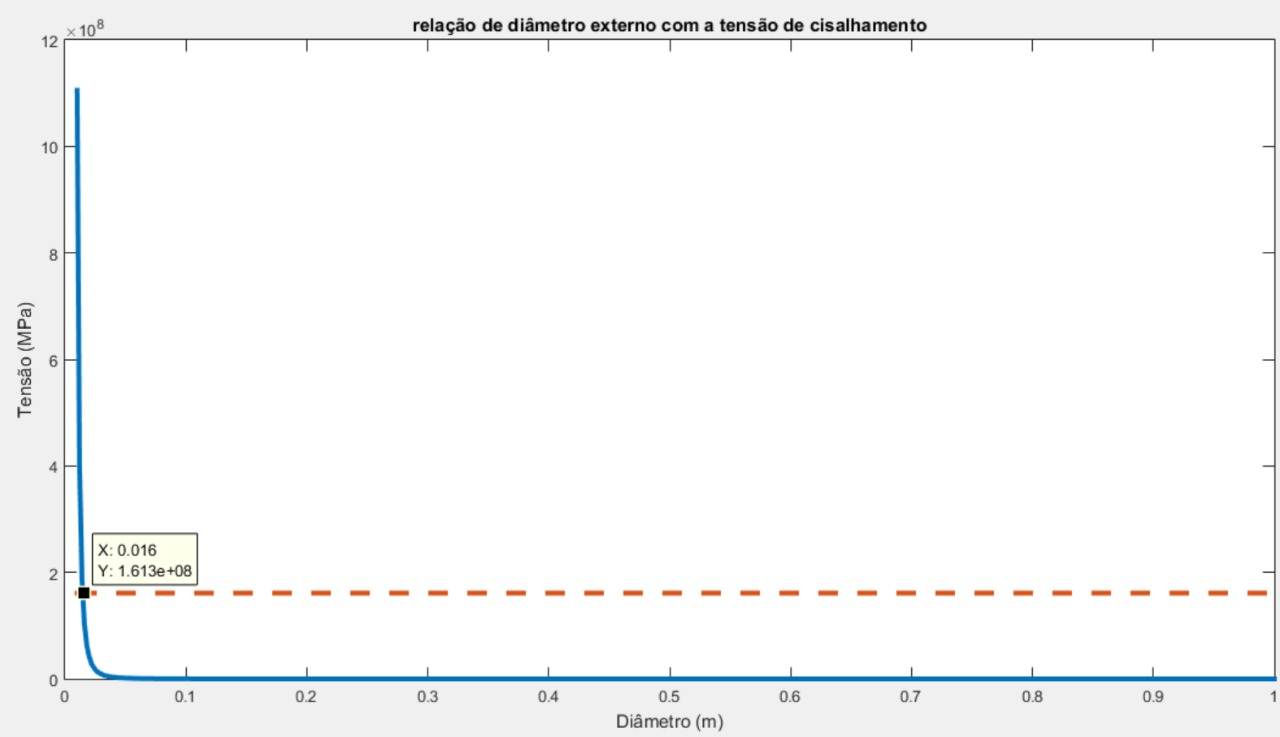
\includegraphics[scale=0.24]{figuras/matlab_hastes.jpg}
            \caption{Definição do diâmetro mínimo das hastes.}
            \label{fig:matlab}
        \end{figure}     

Foi escolhido 2 polegadas por ser comercialmente mais fácil de encontrar.

Analisando a estrutura em \textit{Ansys}, foi possível a obtenção das tensões equivalente de \textit{Von-Mises} e o deslocamento da estrutura, sendo esta máxima em 4mm.

A Figura \ref{fig:presilha} apresenta o local de esforço máximo e o comportamento da tensão nas presilhas que suportam as caixas.

\begin{figure}[H]
	        \centering
            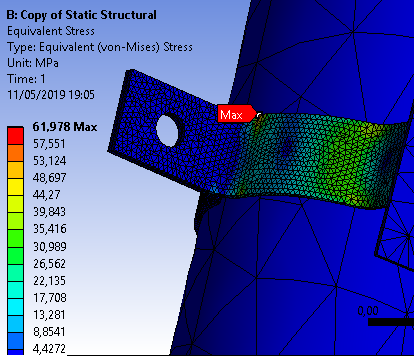
\includegraphics[scale=0.8]{figuras/tension_presilha.PNG}
            \caption{Tensão equivalente de \textit{Von-Mises} para as presilhas.}
            \label{fig:presilha}
            \end{figure}
            
A Figura \ref{fig:defor_painel} apresenta a tensão equivalente de \textit{Von-Mises} para o suporte para o painel solar em relação a deformação.

            \begin{figure}[H]
	        \centering
            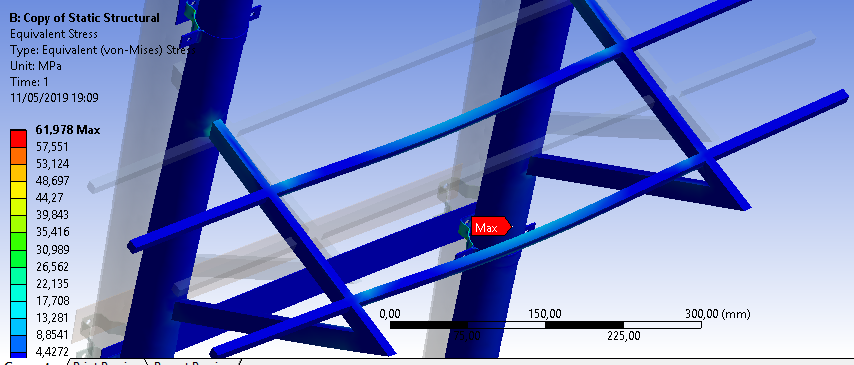
\includegraphics[scale=0.5]{figuras/tensao_relacao_deformacao.PNG}
            \caption{Tensão equivalente de \textit{Von-Mises} para o suporte para o painel solar em relação a deformação.}
            \label{fig:defor_painel}
            \end{figure}
            
\subsection{Dissipação de calor}

Devido ao fato da escolha do material para a estrutura ser metálico e o Brasil ter abundância em incidência solar, deve-se garantir que a temperatura de operação esteja entre 20\% e 30\% abaixo da temperatura limite dos componentes \cite{dissipacao}. Tendo em vista que a temperatura limite de operação é 50$^{\circ}$ a temperatura de operação foi fixada em 36$^{\circ}$ Para modelagem do problema é proposto um ventilador elétrico, para a indução de dissipação por convecção combinada (natural e forçada) \cite{transcal} e dissipador de calor no processador da \textit{Raspberry}, devido à sua maior temperatura de operação.

Com um ventilador de 37 $m^3/h$, foi calculado que a dissipação na direção horizontal (a de maior valor) é de aproximadamente 50W, com um tempo de relaxamento de 45 min.

\section{Projeto dos Componentes Estruturais}

Foram utilizadas no projeto duas caixas de painel de controle (quadro de comando) pois essas possuíam todas as necessidades do projeto, como mostra a Figura \ref{caixa}. As caixas são de aço e possuem 1mm de espessura com dimensões de 500x500x250mm. São rígidas e resistentes a corrosão com tratamento de fosfato de zinco e pintura a pó. Ambas possuem borrachas de vedação hermética e possuem grau de proteção IP54 conforme a ABNT NBR IEC 60529 \cite{involucro}. Cada caixa pesa 10 quilos. Na figura é possível ver a placa de montagem da cor laranja utilizada para acoplar os componentes eletrônicos necessários para o funcionamento do RaDop.

\begin{figure}[H]
	\centering
    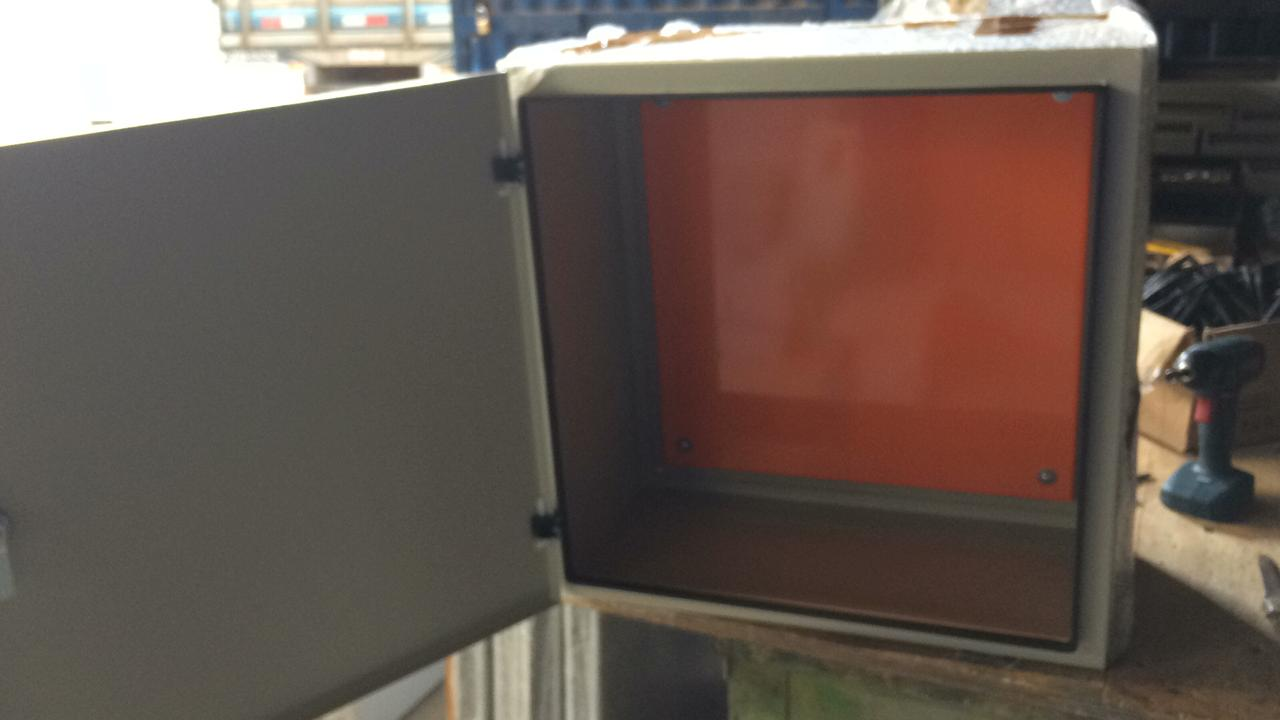
\includegraphics[keepaspectratio=true,scale=0.315]{figuras/caixa.jpg}
    \caption{Caixa de aço utilizada para o projeto.}
    \label{caixa}
\end{figure}

Dois tubos de aço carbono chapa 13 (2,25 mm) com 2 polegadas de diâmetro (50,80 mm) foram utilizadas para suportar todos os módulos necessários da estrutura, suas dimensões foram selecionadas com base nos cálculos numéricos feitos para medir os esforços e tensões que elas são submetidas, como mostra a Figura \ref{tubos}. Os tubos foram selecionadas como base nas suas propriedades de rigidez e o fator comercial também foi algo decisivo na escolha do material. Cada tubo possui 4 metros sendo que 1 metro foi utilizado para que a estrutura tivesse sua fundação no concreto, que é detalhado na próxima seção desse relatório.

\begin{figure}[H]
	\centering
    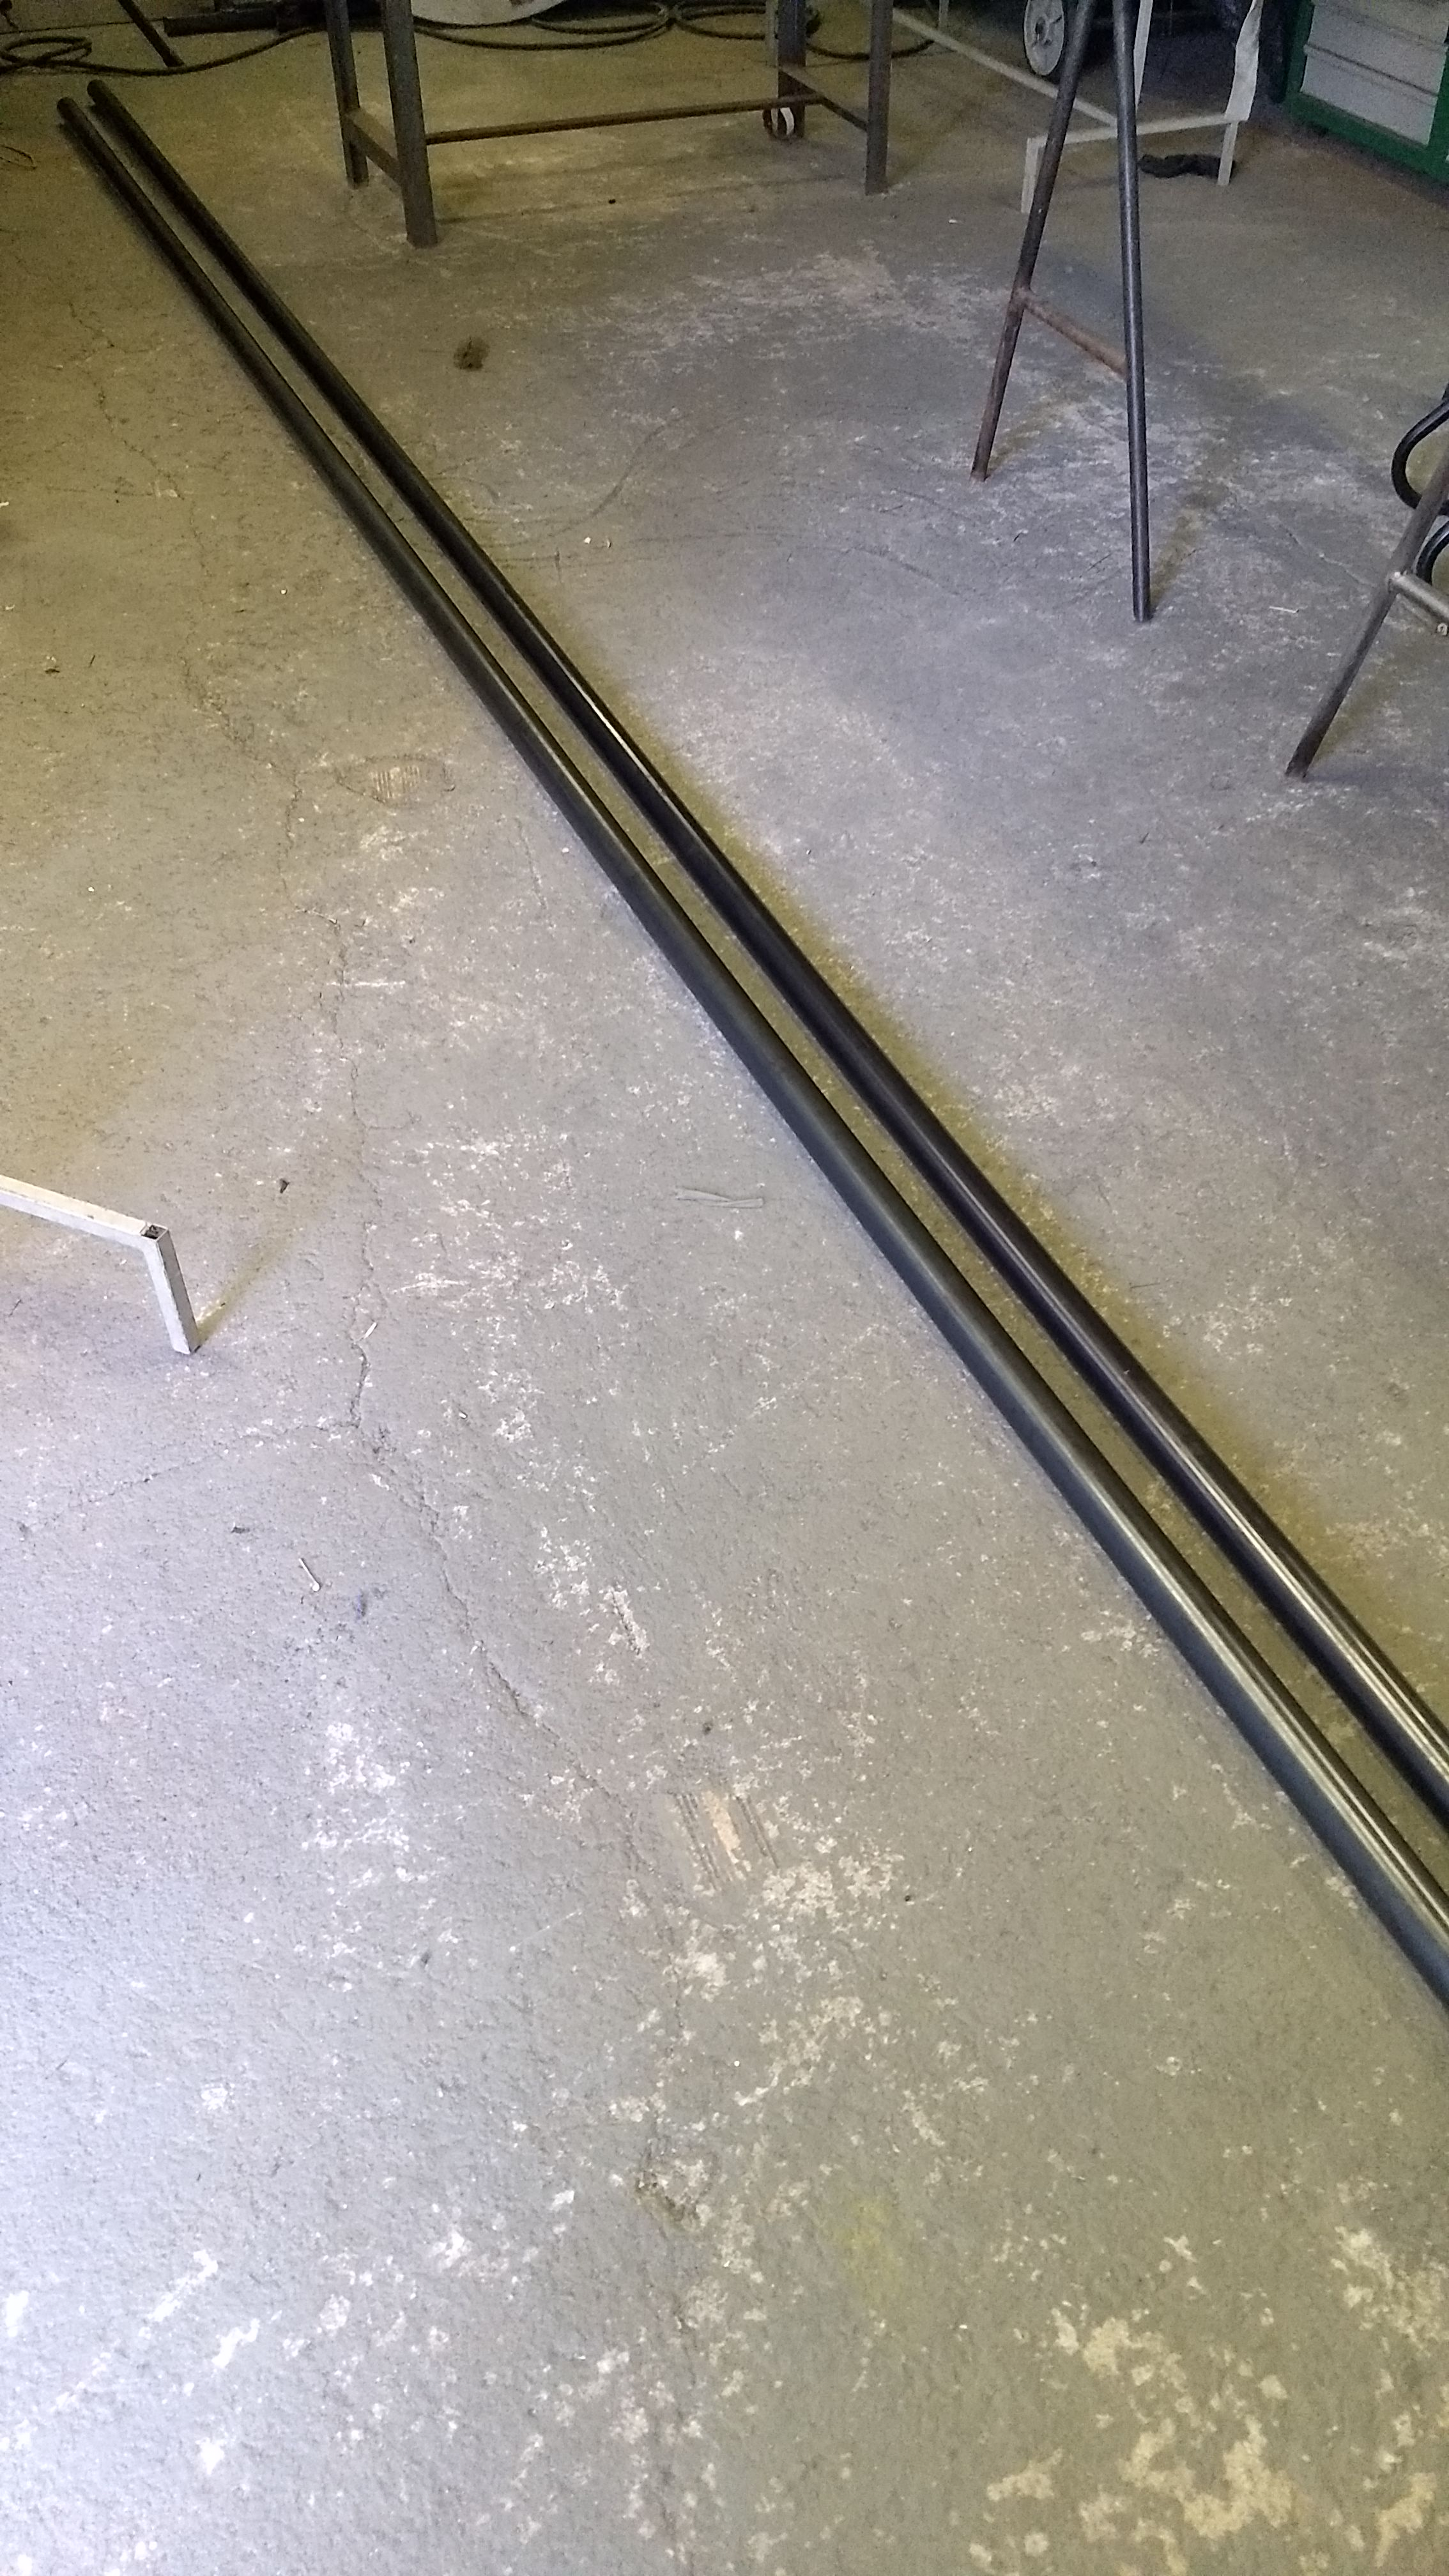
\includegraphics[keepaspectratio=true,scale=0.1,angle=90]{figuras/tubos.jpeg}
    \caption{Tubos de aço carbono chapa 13 utilizada para o projeto.}
    \label{tubos}
\end{figure}

Foram usadas 8 abraçadeiras tipo copo com 1,5 polegadas para prender as caixas nos tubos feitas de aço com 1mm de espessura, como mostra a Figura \ref{abrac}. A utilização das abraçadeiras facilita a manutenção e evita a utilização de solda para fixar as caixas.

\begin{figure}[H]
	\centering
    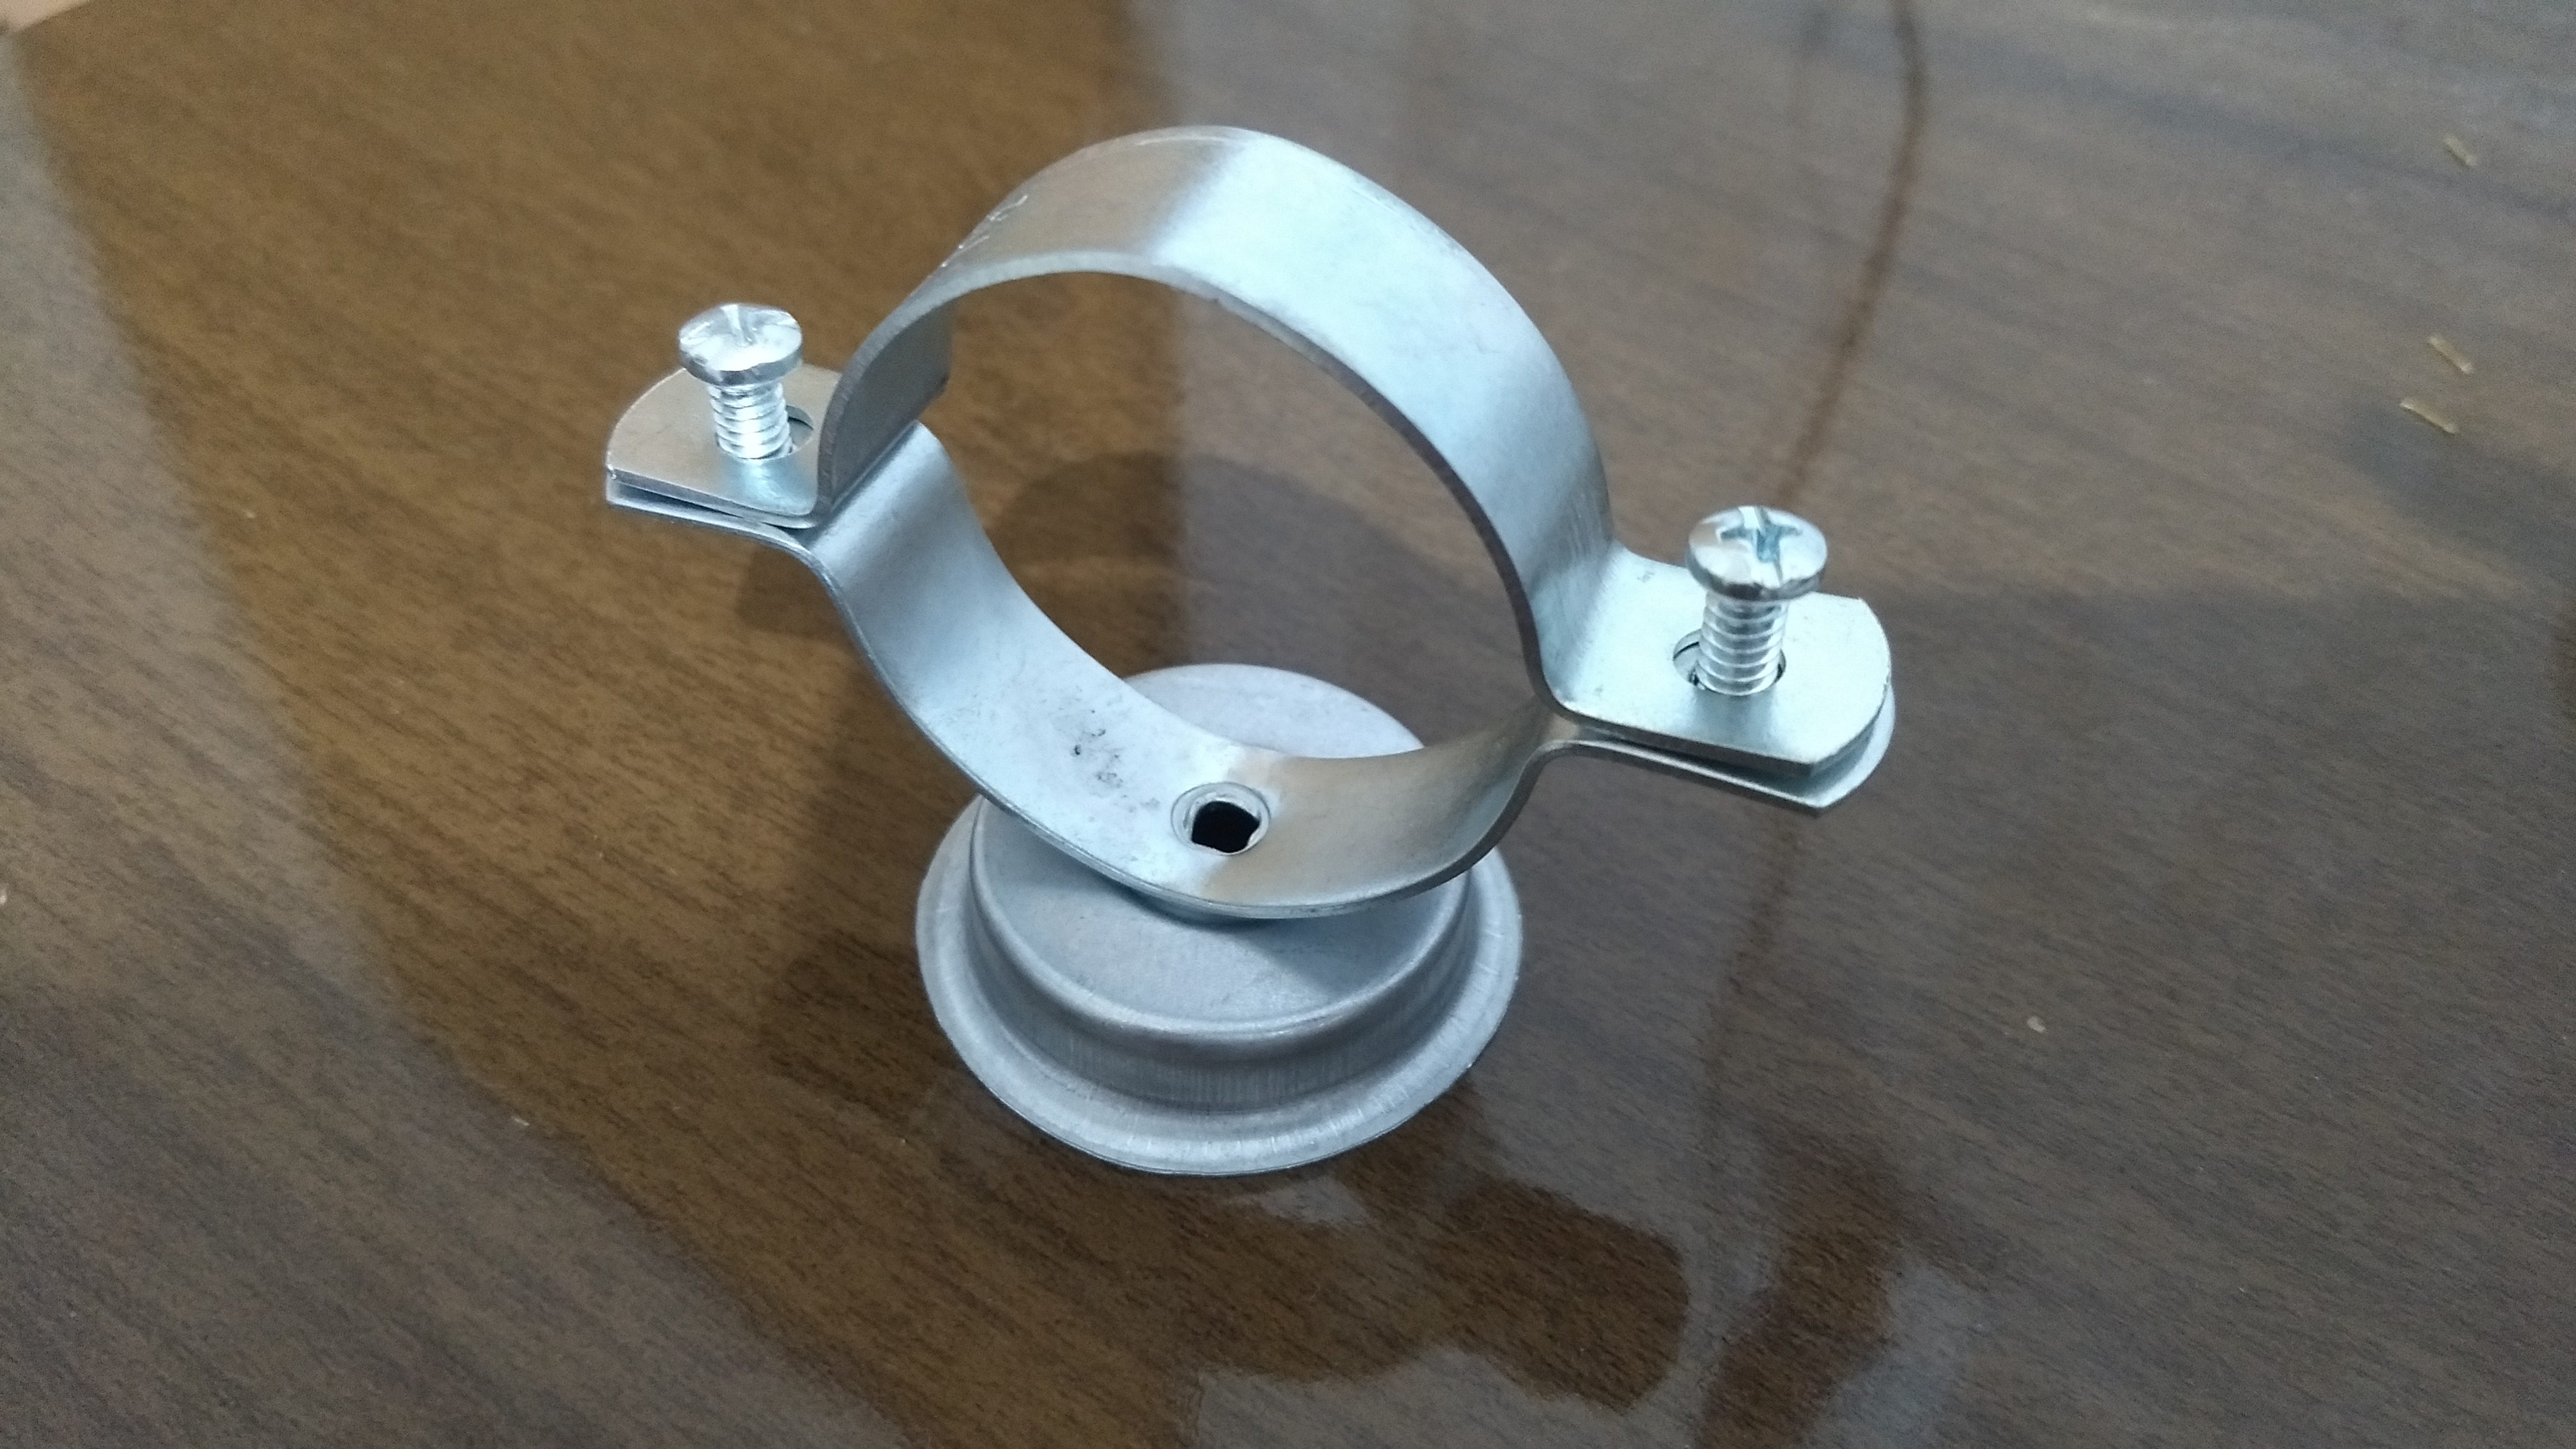
\includegraphics[keepaspectratio=true,scale=0.1]{figuras/abrac.jpg}
    \caption{Caixa de aço utilizada para o projeto.}
    \label{abrac}
\end{figure}

O suporte para o acoplamento dos painéis solares foi feito com tubos quadrados com 20mm de lado e 1,25mm de espessura de parede, como mostra a Figura \ref{tuboquad}. Foi decidido a utilização do tubo quadrado pois esse resiste melhor a flexão, que surgi devido ao peso dos painéis solares após a instalação. Foram utilizados parafusos do tipo M6 para fixar os painéis e não permitir a queda dos mesmos.

\begin{figure}[H]
	\centering
    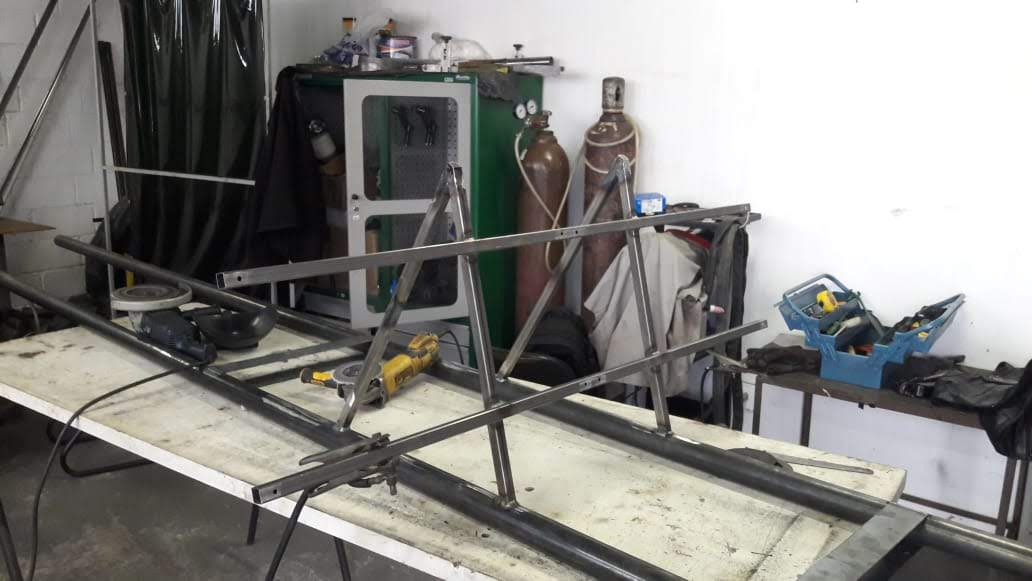
\includegraphics[keepaspectratio=true,scale=0.43]{figuras/suportepainel1.jpg}
    \caption{Suporte para o acoplamento dos painéis solares feito com tubos quadrados.}
    \label{tuboquad}
\end{figure}


\section{Construção do Protótipo}

O projeto foi construído utilizando os recursos disponibilizados pela Universidade de Brasília com o galpão, seu maquinário e os técnicos disponíveis. As escolhas dos materiais e processos de fabricação foram feitas através do conhecimento prévio adquirido através das simulações computacionais.

Inicialmente o projeto começou com a construção do suporte principal, as hastes de aço carbono. Assim foram soldados as chapas chatas entre os tubos nas dimensões corretas para criar o que seria a base de sustentação de todos os demais componentes, estruturais ou eletrônicos. 

\begin{figure}[H]
	\centering
    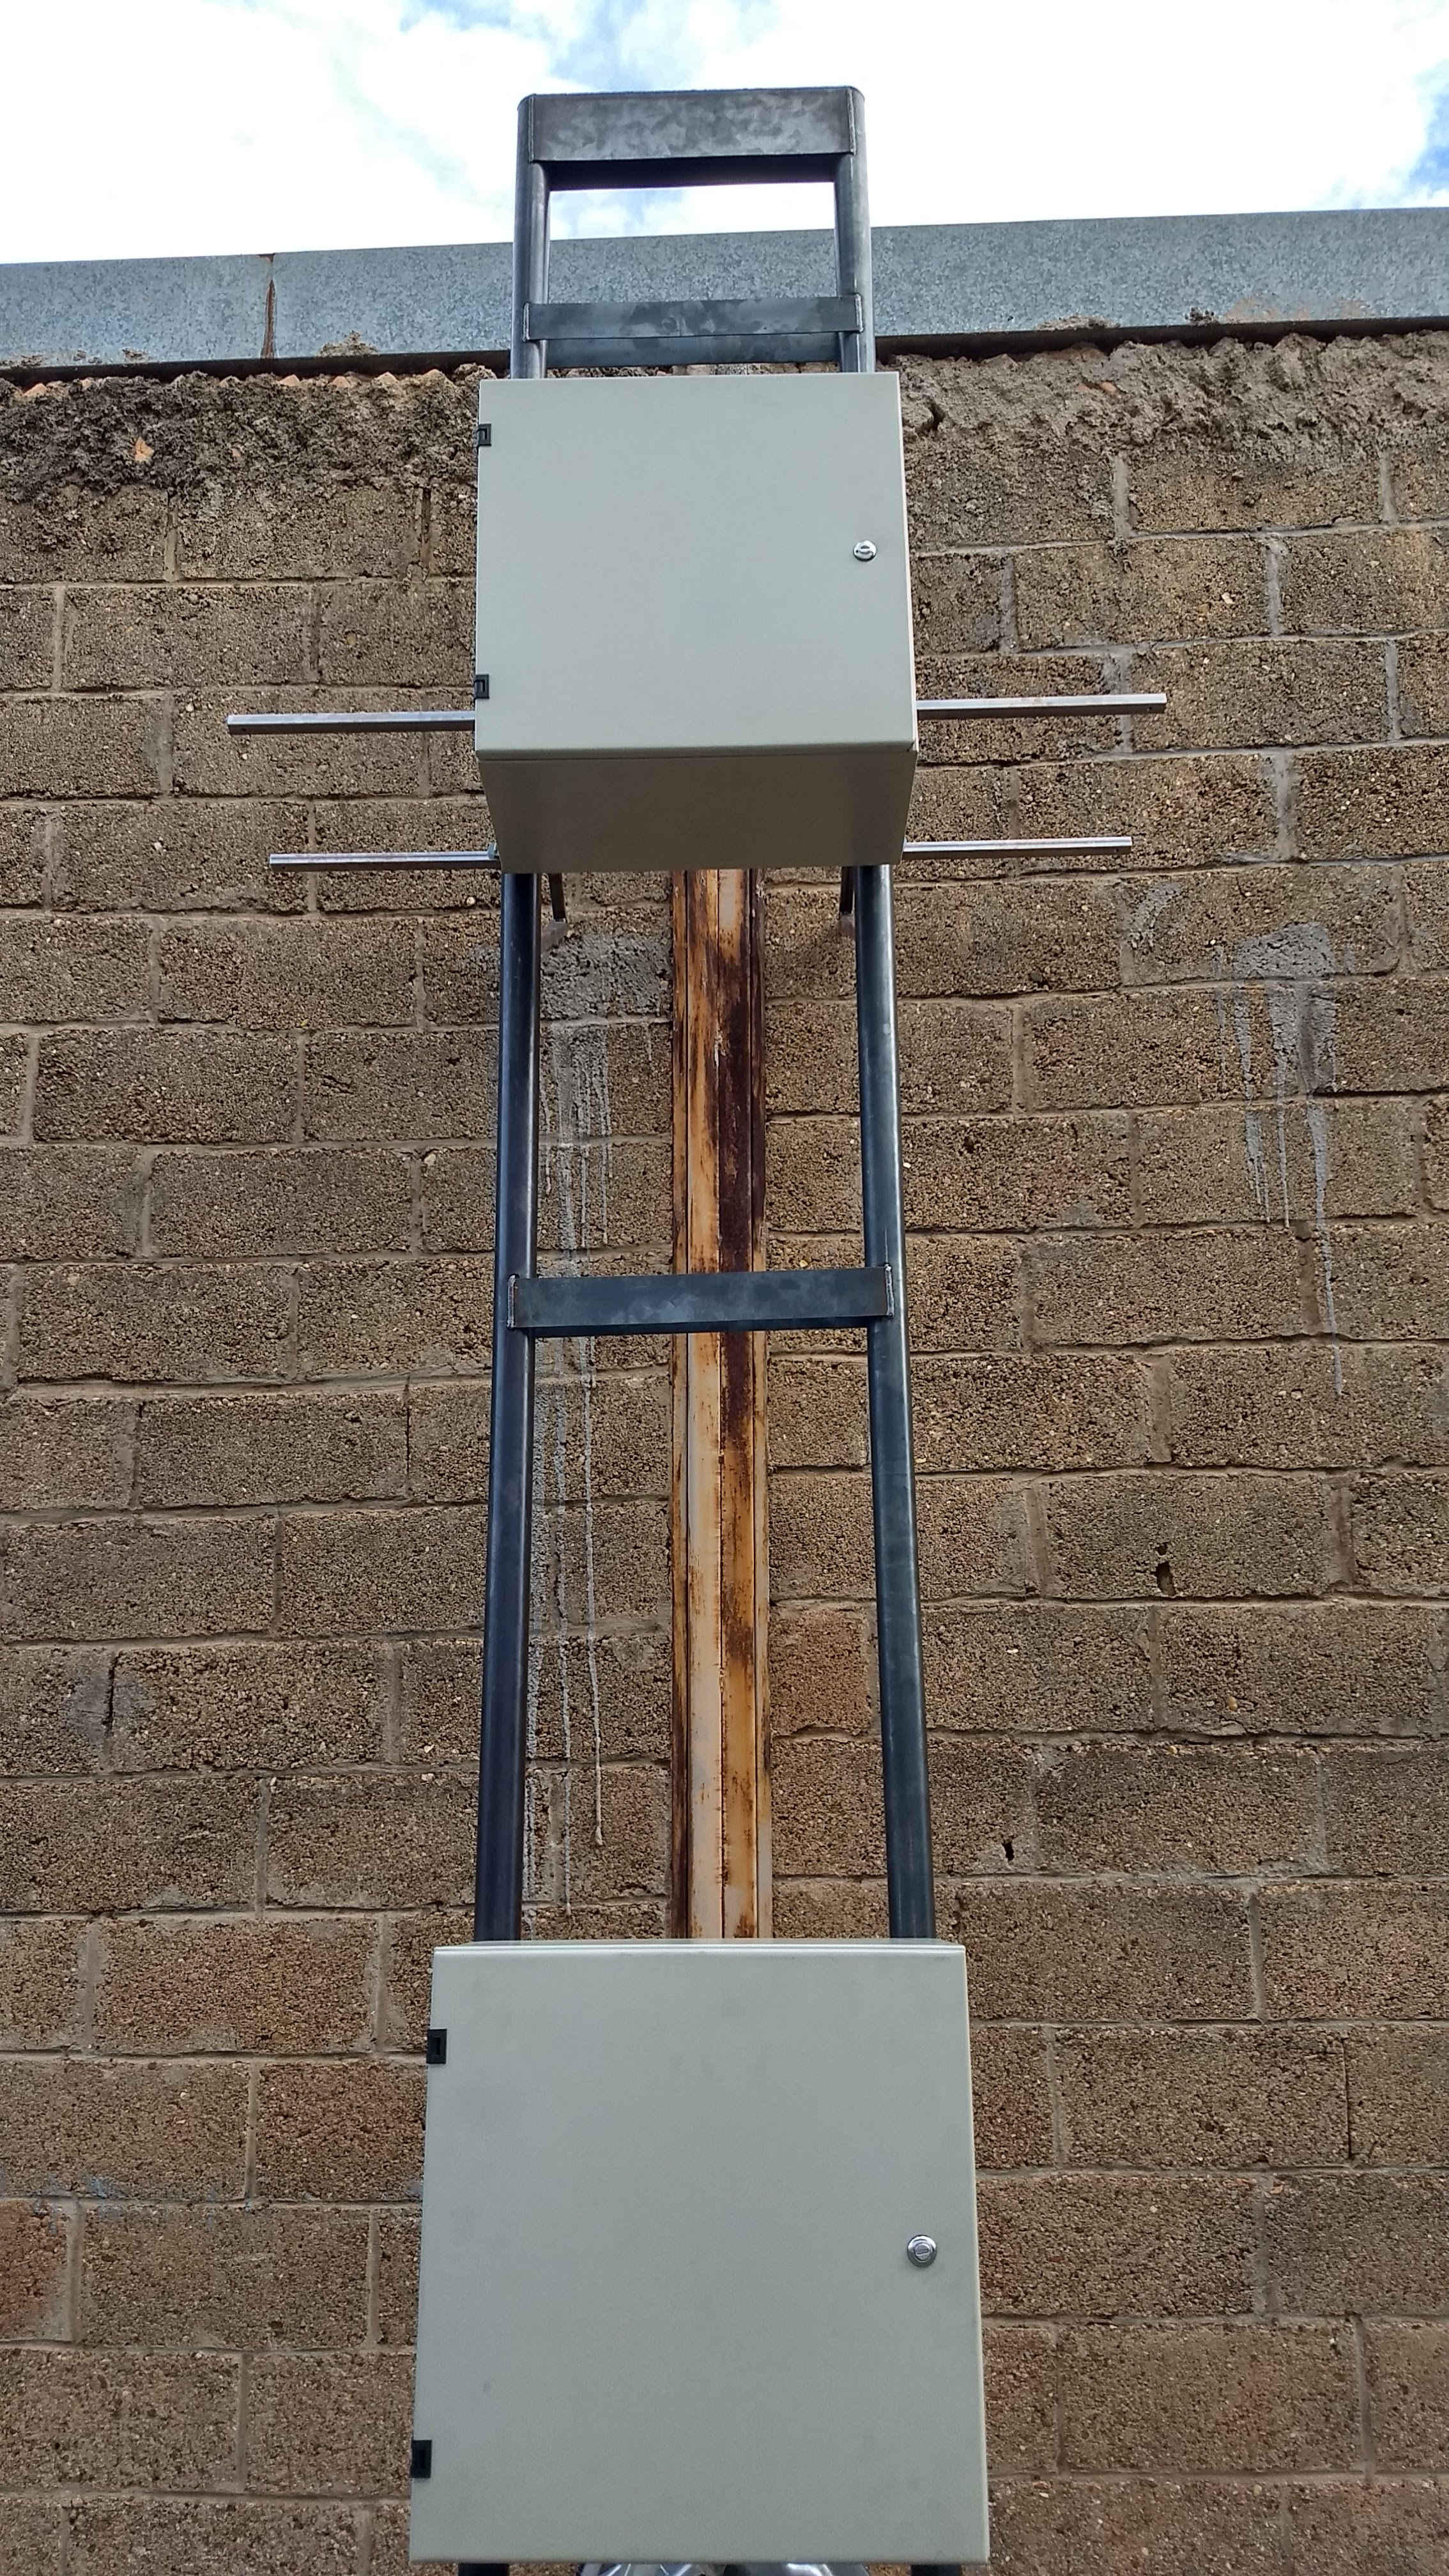
\includegraphics[keepaspectratio=true,scale=0.12]{figuras/estrucomp1.jpg}
    \caption{Hastes construídas em aço carbono.}
    \label{hastescons}
\end{figure}

Com as hastes prontas foi então construído o último módulo que seria soldado, o suporte para os painéis solares. O corte dos tubos quadrados nas dimensões necessárias foram realizados para então soldar junto as hastes da estrutura. Os furos para o encaixe dos painéis solares também foram feitos no suporte.

\begin{figure}[H]
	\centering
    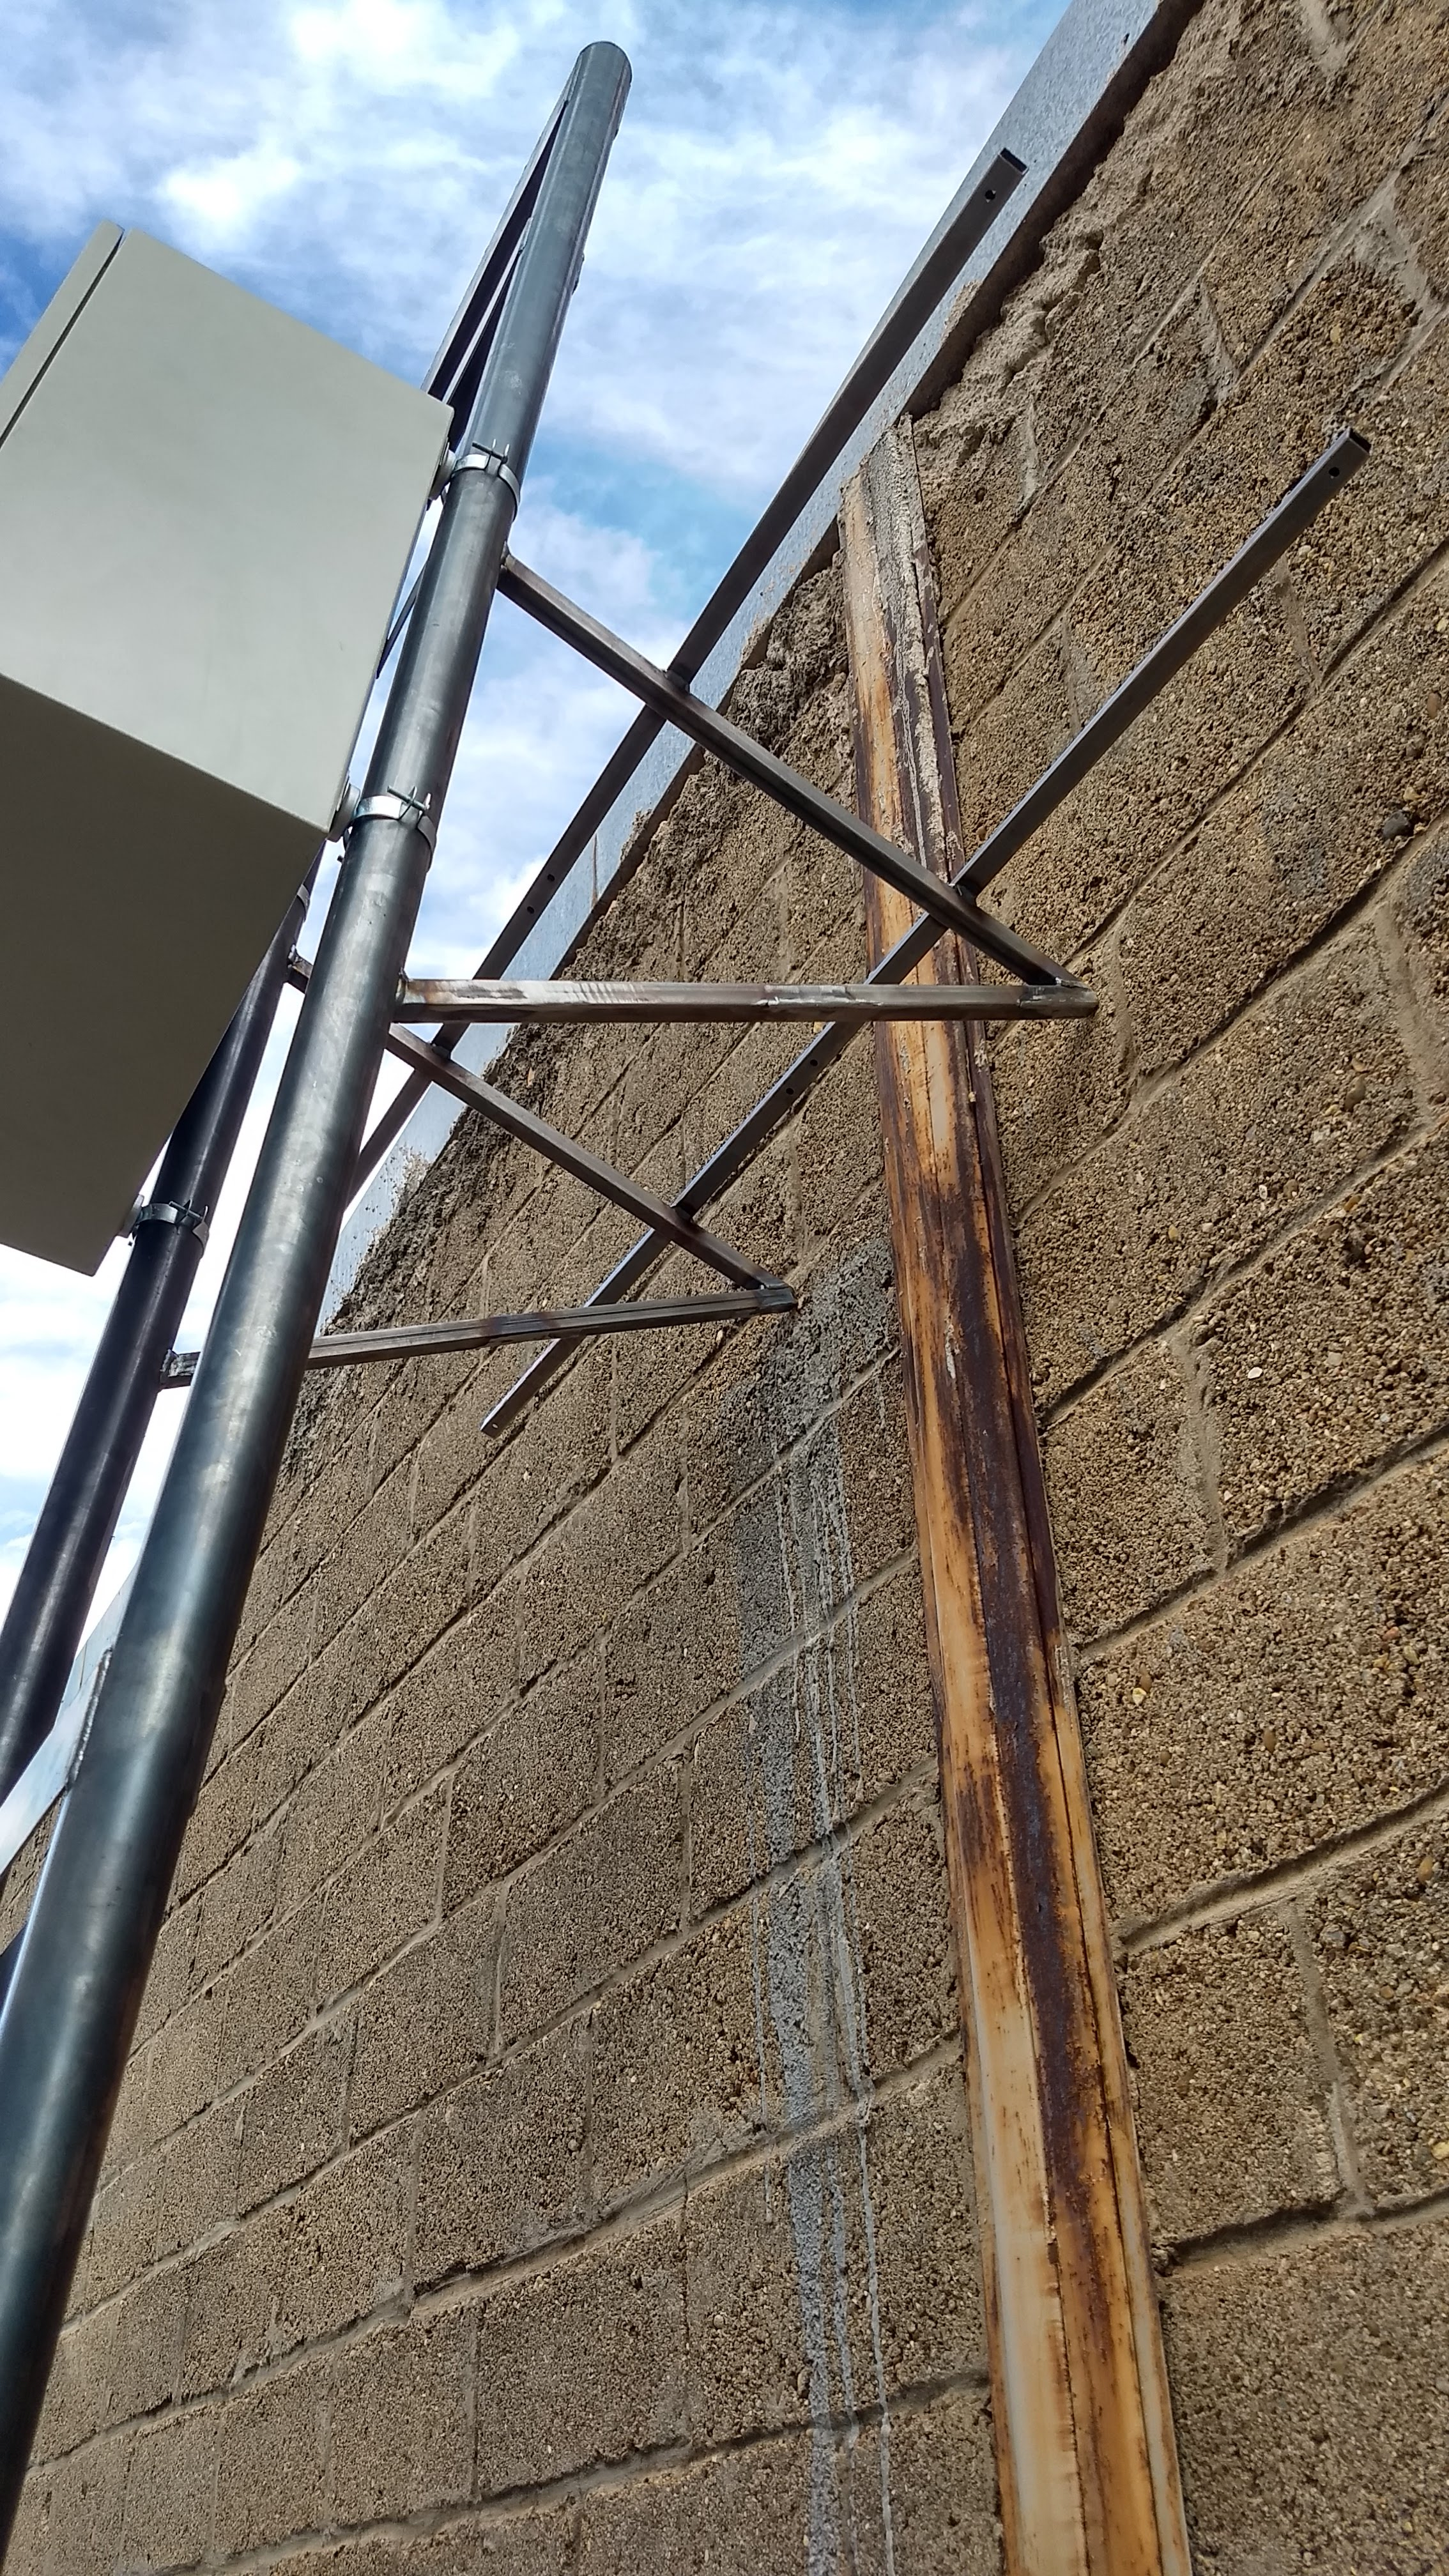
\includegraphics[keepaspectratio=true,scale=0.12]{figuras/suportepainel2.jpg}
    \caption{Suporte dos painéis solares construídas tubos quadrados de aço carbono com 20x20mm.}
    \label{supaisolcons}
\end{figure}

Com as abraçadeiras fixadas na hastes foram feitos os furos nas placas chatas (que distribuem o peso das caixas) e nas caixas superior e inferior. Utilizando parafusos e porcas do tipo M6, foram fixadas as caixas nas alturas pré-determinadas pelos desenhos técnicos. 

\begin{figure}[H]
	\centering
    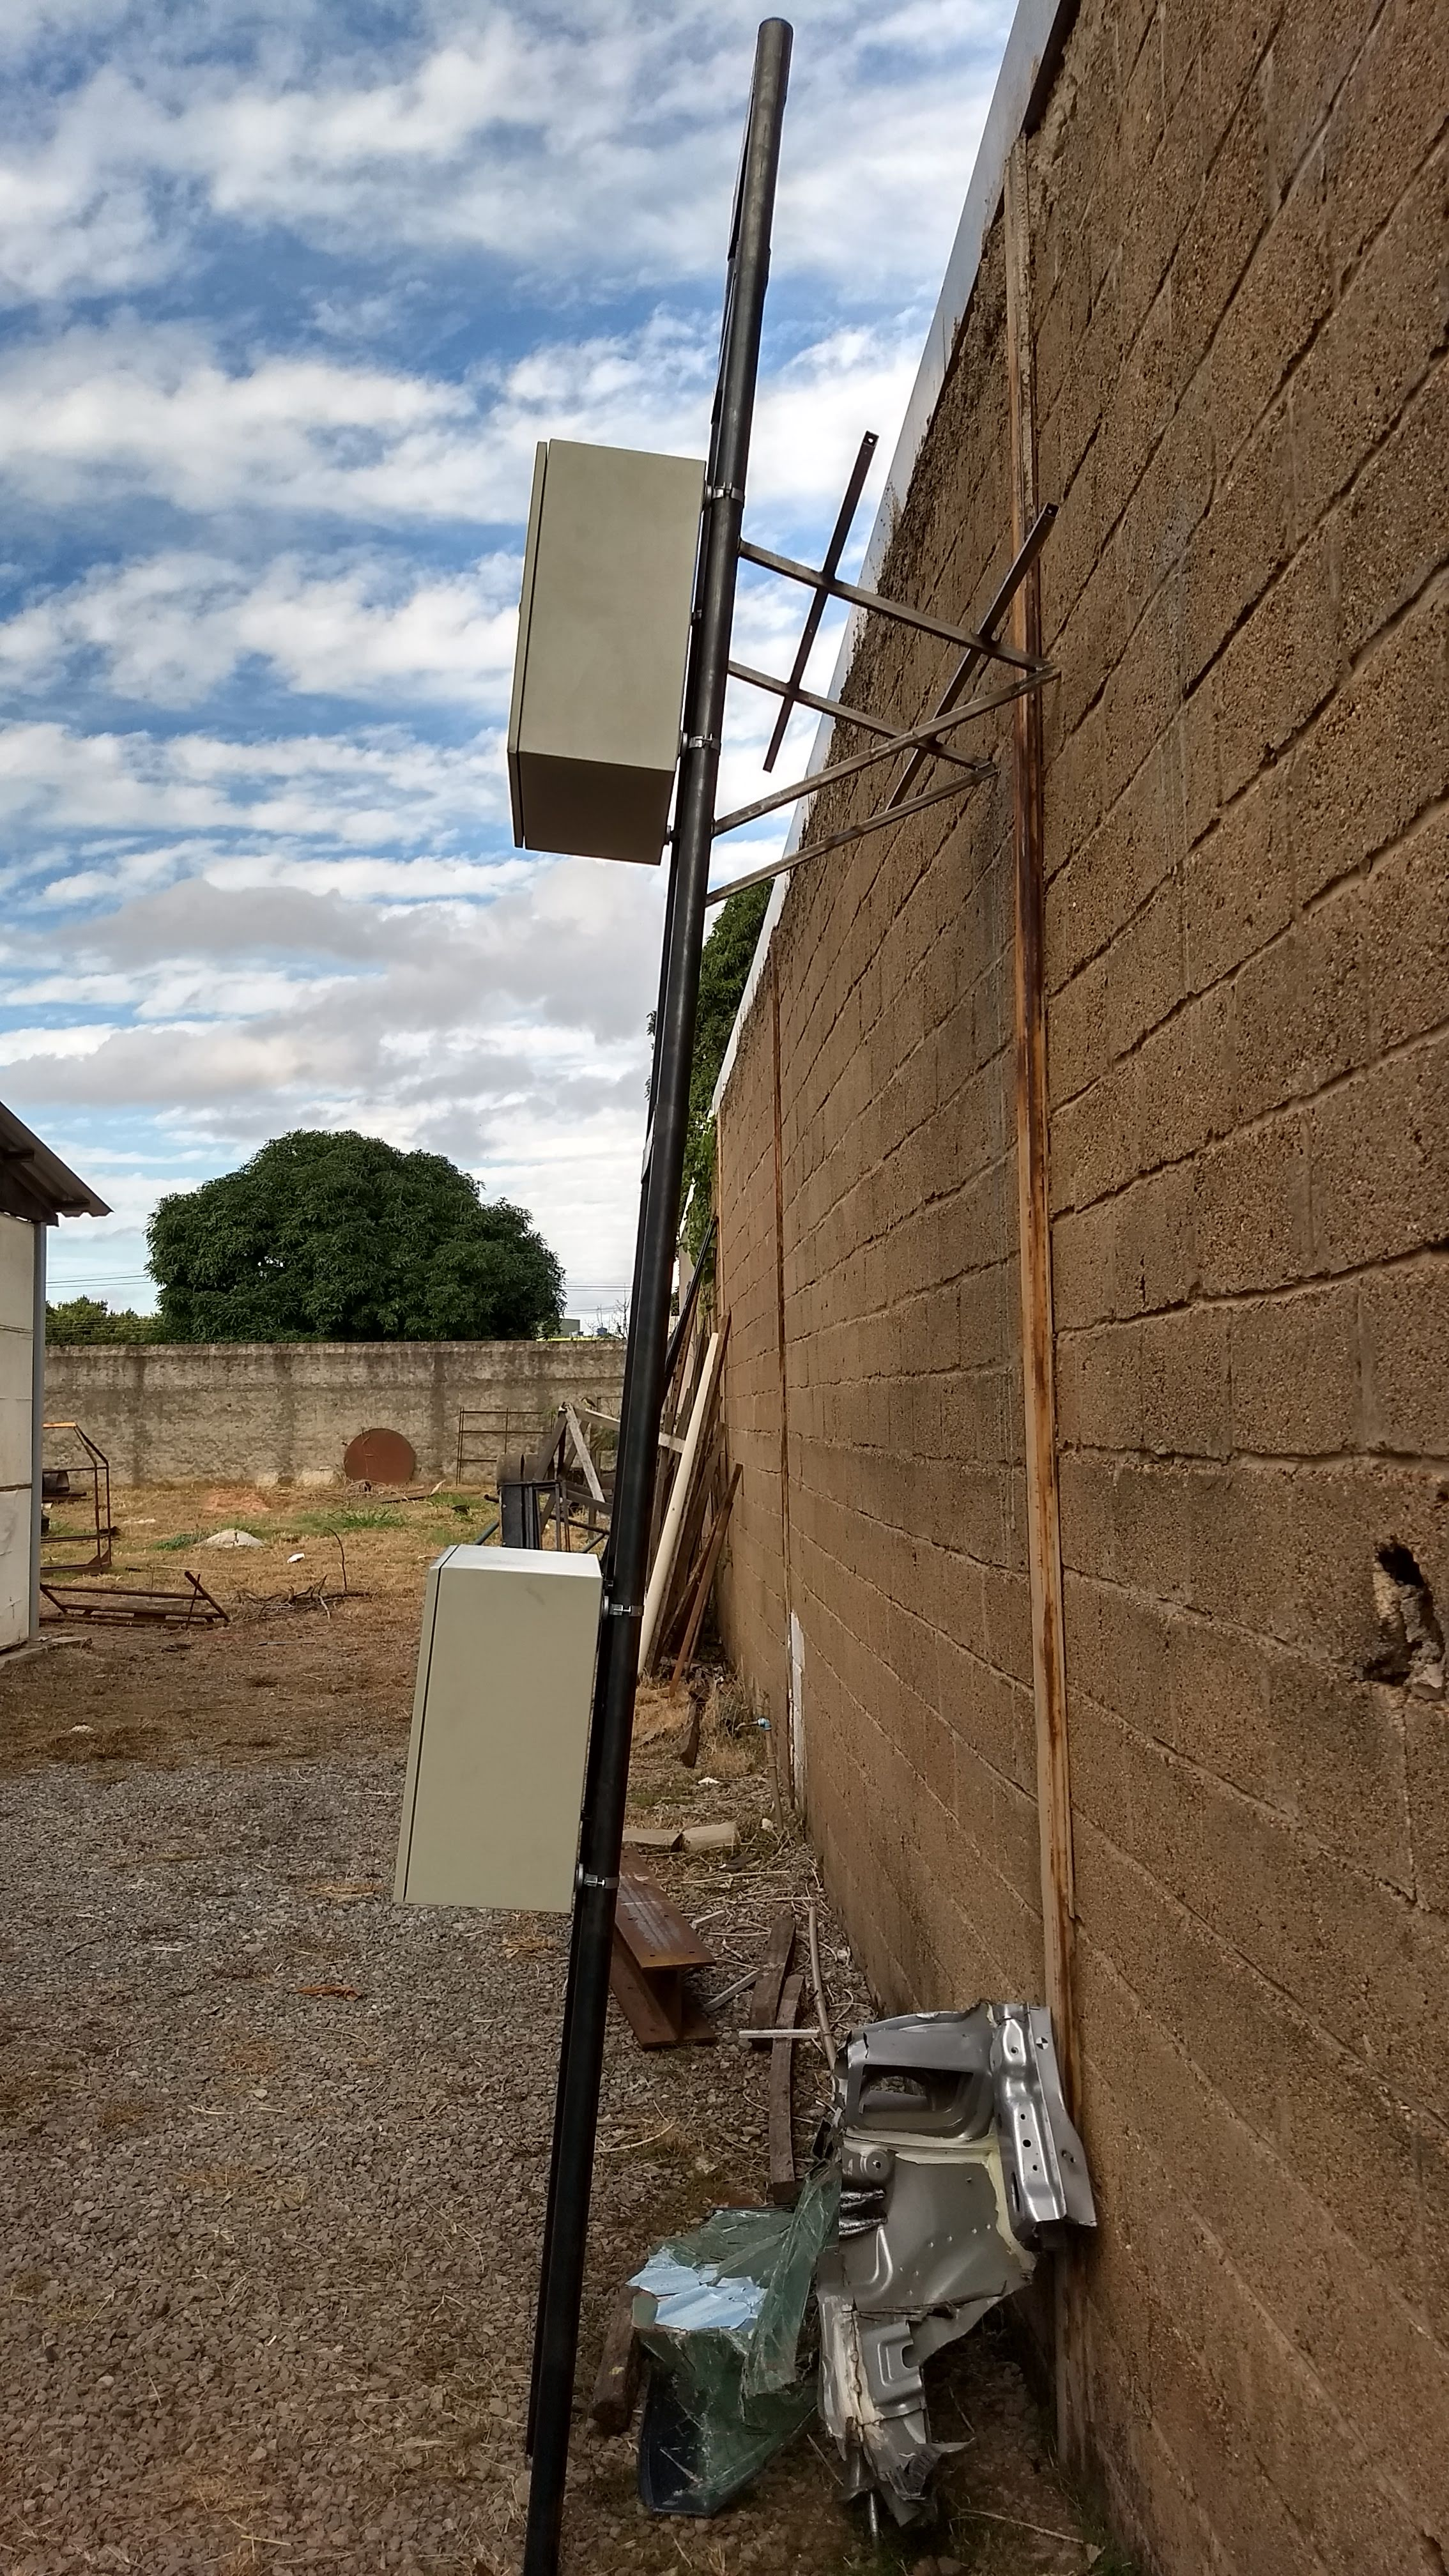
\includegraphics[keepaspectratio=true,scale=0.12]{figuras/estrucomp2.jpg}
    \caption{Caixa acoplada utilizando as abraçadeiras nas hastes.}
    \label{caixaacop}
\end{figure}


A fundação foi pensada para proporcionar maior estabilidade para a estrutura. Ter uma fundação faz com que o protótipo esteja muito mais perto da situação do produto real. Através do aval dos responsáveis na Universidade de Brasília, foi possível a construção de uma fundação de concreto no estacionamento para teste e apresentação do projeto para os professores avaliadores. 

As dimensões escolhidas para a construção da fundação são de 40x70cm na superfície e 1 metro de profundidade abaixo do chão. Levando em consideração que 1 metro da estrutura (as hastes) é encaixada na fundação é possível garantir a estabilidade necessária para a estrutura. A figura \ref{fund} mostra como ficou a fundação após a construção da mesma.

\begin{figure}[H]
	\centering
    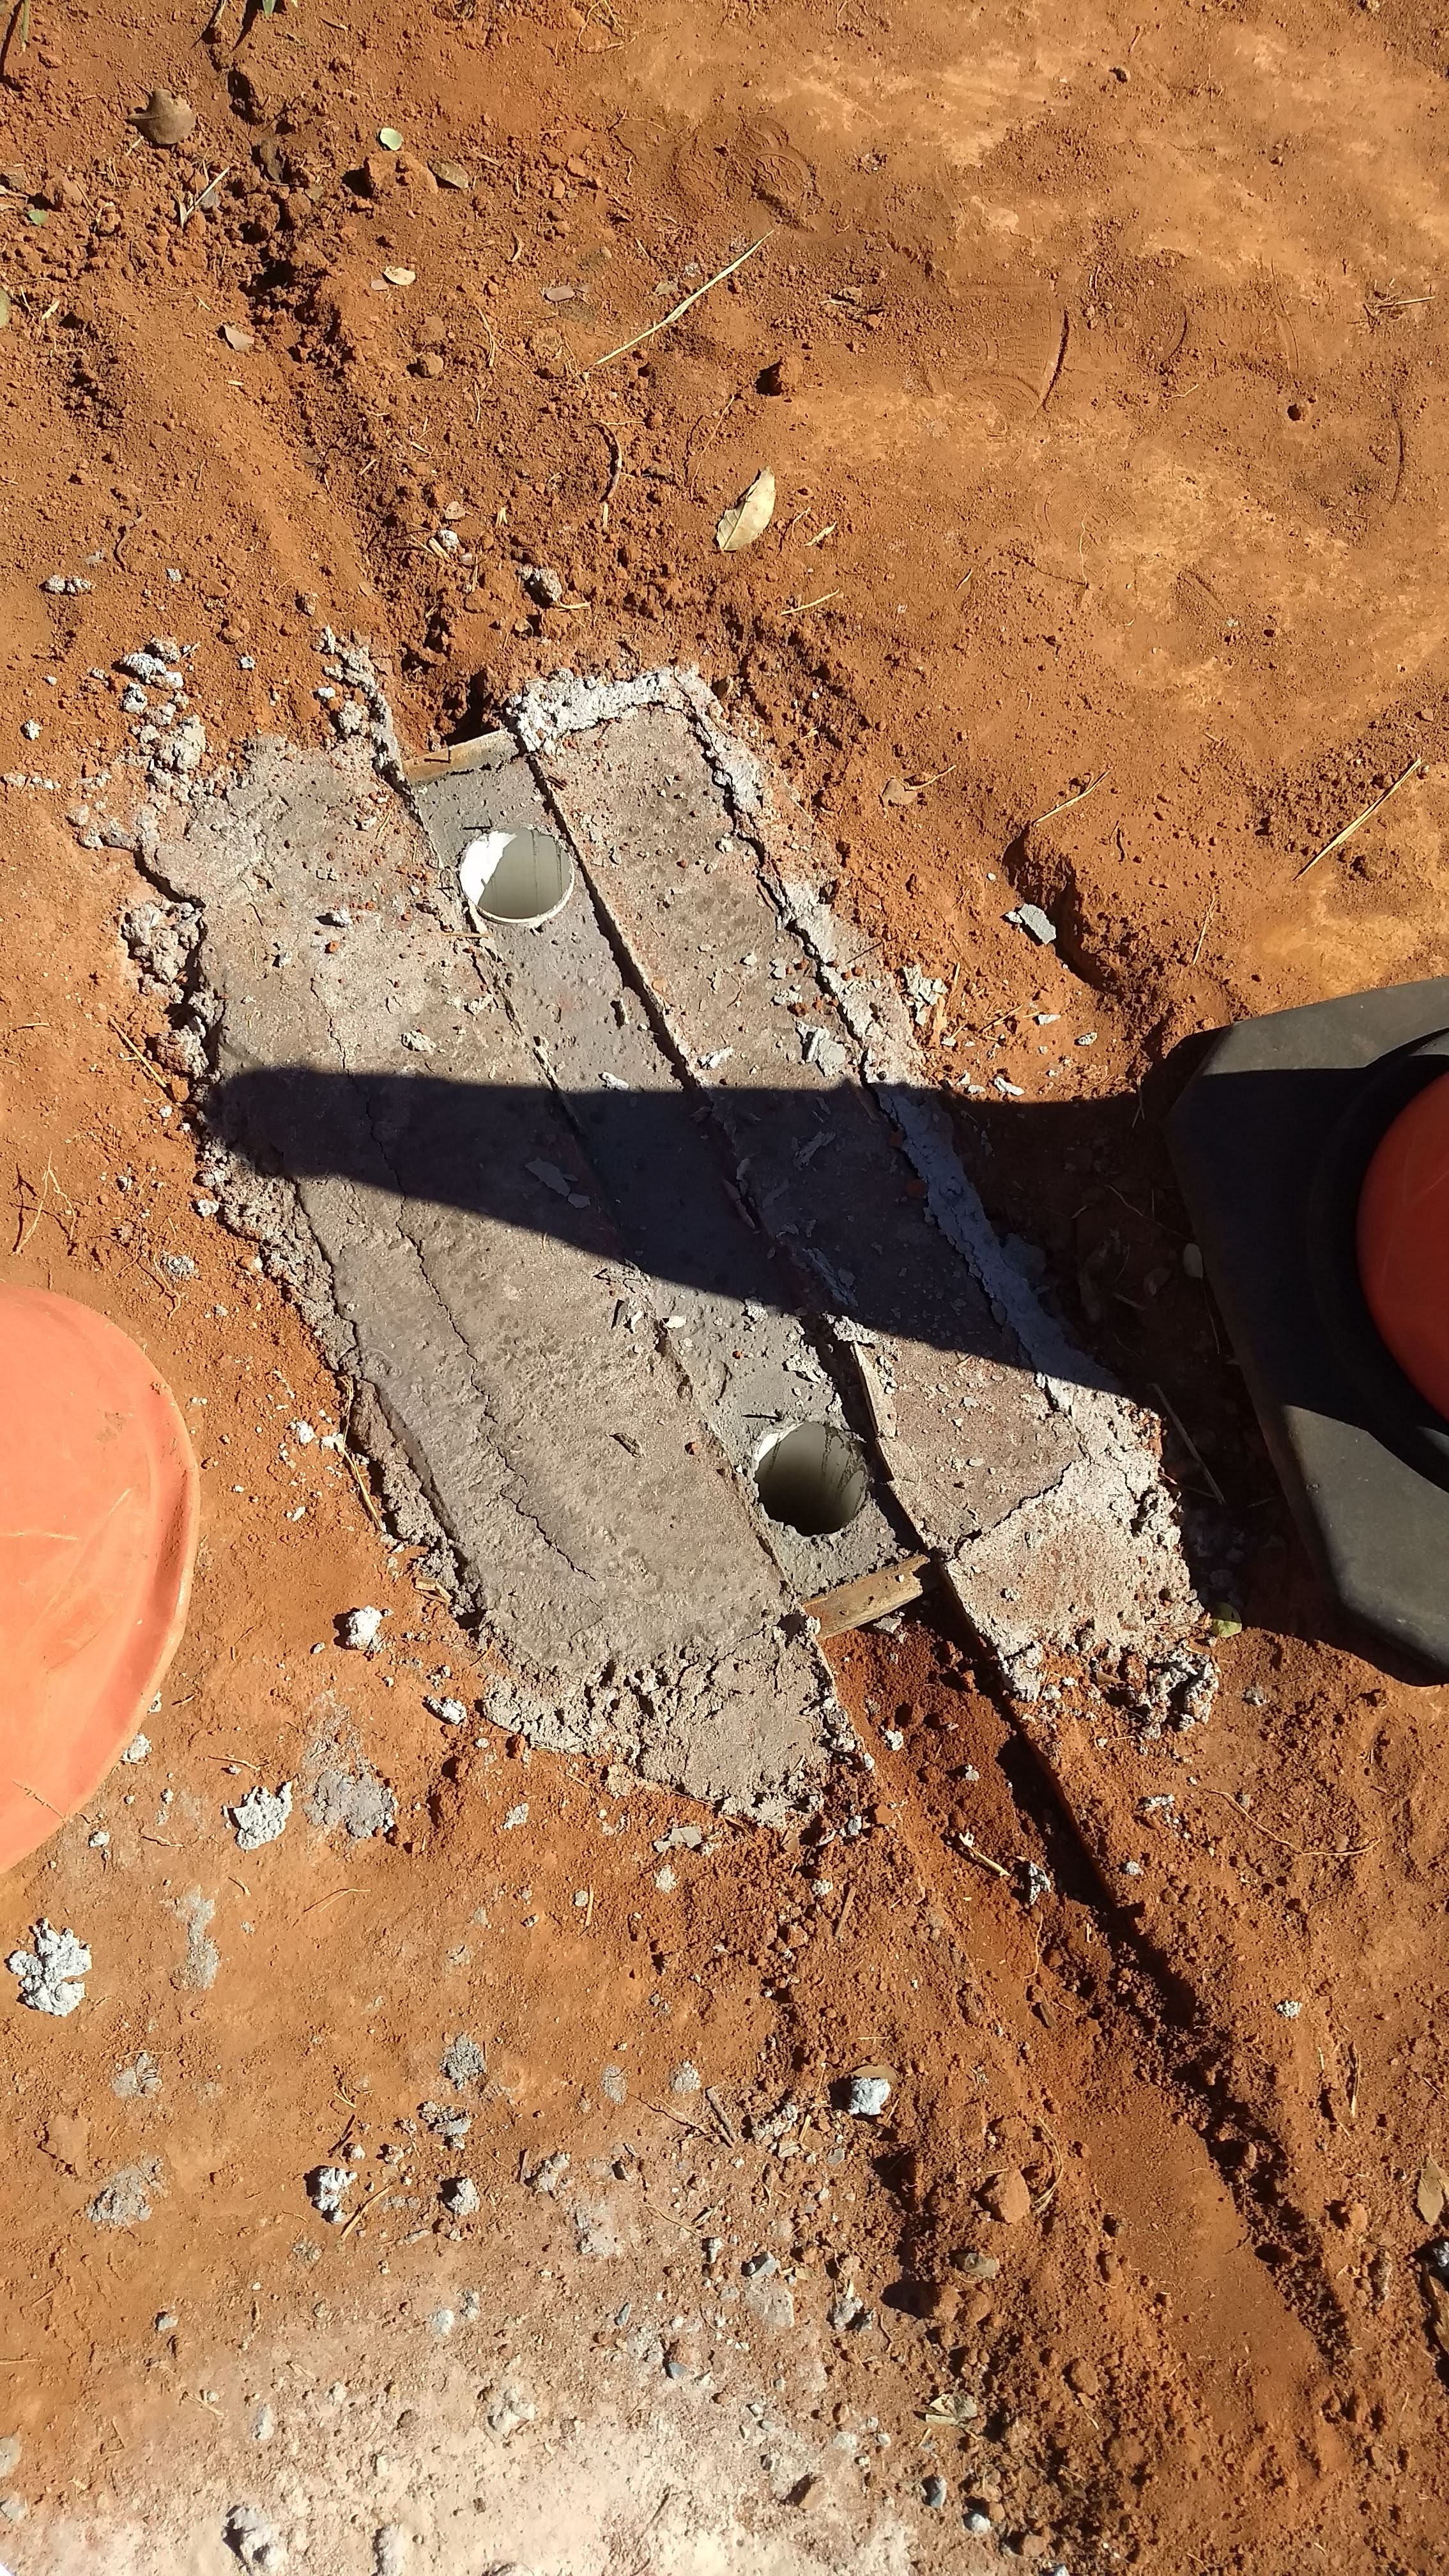
\includegraphics[keepaspectratio=true, angle=90, scale=0.11]{figuras/fund.jpg}
    \caption{Fundação de concreto feita para melhor estabilidade da estrutura.}
    \label{fund}
\end{figure}

O local escolhido em comum acordo entres os diretores técnicos de cada subsistema proporciona um teste com melhor acurácia e mais próximo possível da realidade do problema no qual o RaDop se propõe em resolver. 


\section{Teste do Protótipo}

Com a estrutura pronta testes de choques mecânicos foram realizados. A estrutura foi movimentada bruscamente para ter verificar a capacidade das abraçadeiras de suportar o peso das caixas, principalmente a superior já que a inferior está apoiada no chão (fundação) e não é solicitada em termos de esforços significativos.

As portas foram testadas para verificar se a aberturas das mesmas se davam de forma facilitada ou não. Através dos choques mecânicos realizados com a estrutura em sua posição real foram verificadas as soldas realizadas para ver se alguma ruptura havia acontecido e se o sistema poderia ser comprometido por isso.

A estrutura foi posta em inclinação para testar a possibilidade de deflexão nas hastes assim como a possibilidade de ruptura das abraçadeiras.

\section{Avaliação dos Resultados}

Através dos testes realizados a estrutura se mostrou estável. Não foi encontrado nenhuma ruptura de solda mesmo após os choques mecânicos realizados. As abraçadeiras suportaram e não mostraram nenhum sinal de mal funcionamento. As caixas se mostraram eficientes e capazes de realizar seu papel de assegurar o funcionamento dos componentes dos demais subsistemas do projeto.

Sendo assim é possível afirmar que não foi possível verificar nenhum problema que coloque a estrutura parcial ou completamente em risco de ruptura e mal funcionamento. Foi então confirmado experimentalmente os dados obtidos pelas simulações realizadas nas etapas anteriores do projeto.

\section{Projeto de Integração}

A integração se deu mediante ao processo de verificação das necessidades do RaDop. A estrutura buscou atender as necessidades dos demais subsistemas para o funcionamento de maneira adequada do projeto. Várias frentes de operações foram montadas para construir e montar a estrutura final. A integração de estrutura com eletrônica e energia foi feita utilizando-se o espaço do galpão da Universidade de Brasília.

O subsistema de eletrônica utilizou uma placa de montagem da caixa (painel de controle) para acoplar os componentes eletrônicos, sempre pensando na melhor localização dos componentes para posteriormente fazer a fiação necessária. A integração com o subsistema de energia se deu com o acoplamento dos painéis solares no suporte destinado a eles e das baterias na caixa inferior. 

Juntos com todo esse processo foi feita a fiação para conectar os componentes do RaDop. Foi utilizado eletrodutos corrugados e flexíveis (figura \ref{eletrodutos}) e com base nas normas foi visto que era necessário que a fiação ocupasse apenas 40\% da seção transversal do eletroduto, sendo assim foi escolhido eletrodutos com 1 (uma) polegada. A escolha do eletroduto flexível visou a facilidade de adaptar esse tipo de eletrodutos na estrutura. Pensando na possibilidade de uma eventual manutenção não foram utilizadas bocais para os eletrodutos já que os mesmo poderia dificultar a manutenção do protótipo.

\begin{figure}[H]
	\centering
    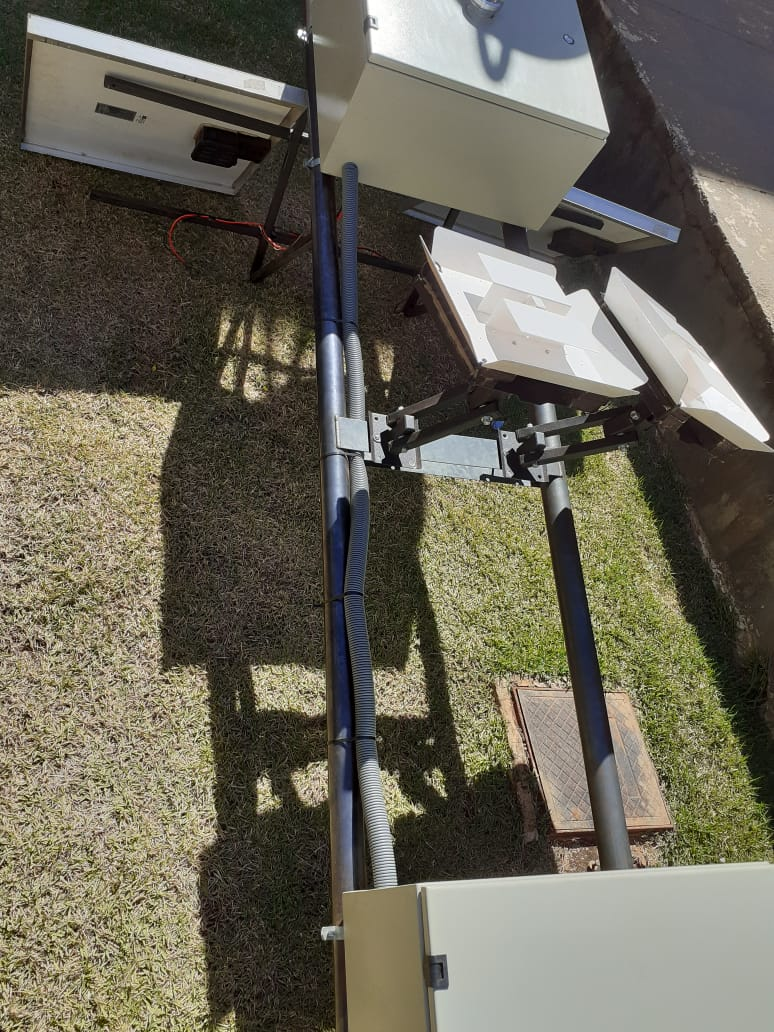
\includegraphics[keepaspectratio=true, scale=0.5]{figuras/eletroduto.jpeg}
    \caption{Eletrodutos corrugados e flexíveis utilizados para a fiação do RaDop.}
    \label{eletrodutos}
\end{figure}

Para esse processo de fiação da estrutura foi necessário fazer dois furos na caixa superior, na parte superior e na parte inferior, e na caixa inferior na parte superior. Com esse arranjo foi possível passar a fiação das baterias que estavam na caixa inferior para o controlador dentro da caixa superior que estava ligado aos painéis solares. Com o furo na parte superior da caixa superior foi possível passar a fiação para os radares e câmera. Foi utilizado um eletroduto corrugado e flexível para isso.

Os desenhos técnicos atualizados se encontram no Apêndice \ref{plantas_construcao} para a melhor verificação da estrutura final que foi feita após o processo de integração com os demais subsistemas.
